\documentclass[tikz,border=6mm]{standalone}
\usepackage{amsmath,amssymb}
\usepackage{fontspec}

\usetikzlibrary{positioning,arrows.meta,shapes.geometric,fit,backgrounds,calc}

% Define cohesive color palette
\definecolor{navyblue}{RGB}{30, 60, 105}
\definecolor{tealblue}{RGB}{20, 110, 105}
\definecolor{purplecat}{RGB}{95, 45, 120}
\definecolor{ambergold}{RGB}{180, 85, 15}
\definecolor{forestgreen}{RGB}{25, 115, 60}
\definecolor{crimsonred}{RGB}{175, 40, 40}
\definecolor{slategrey}{RGB}{70, 85, 100}

\begin{document}
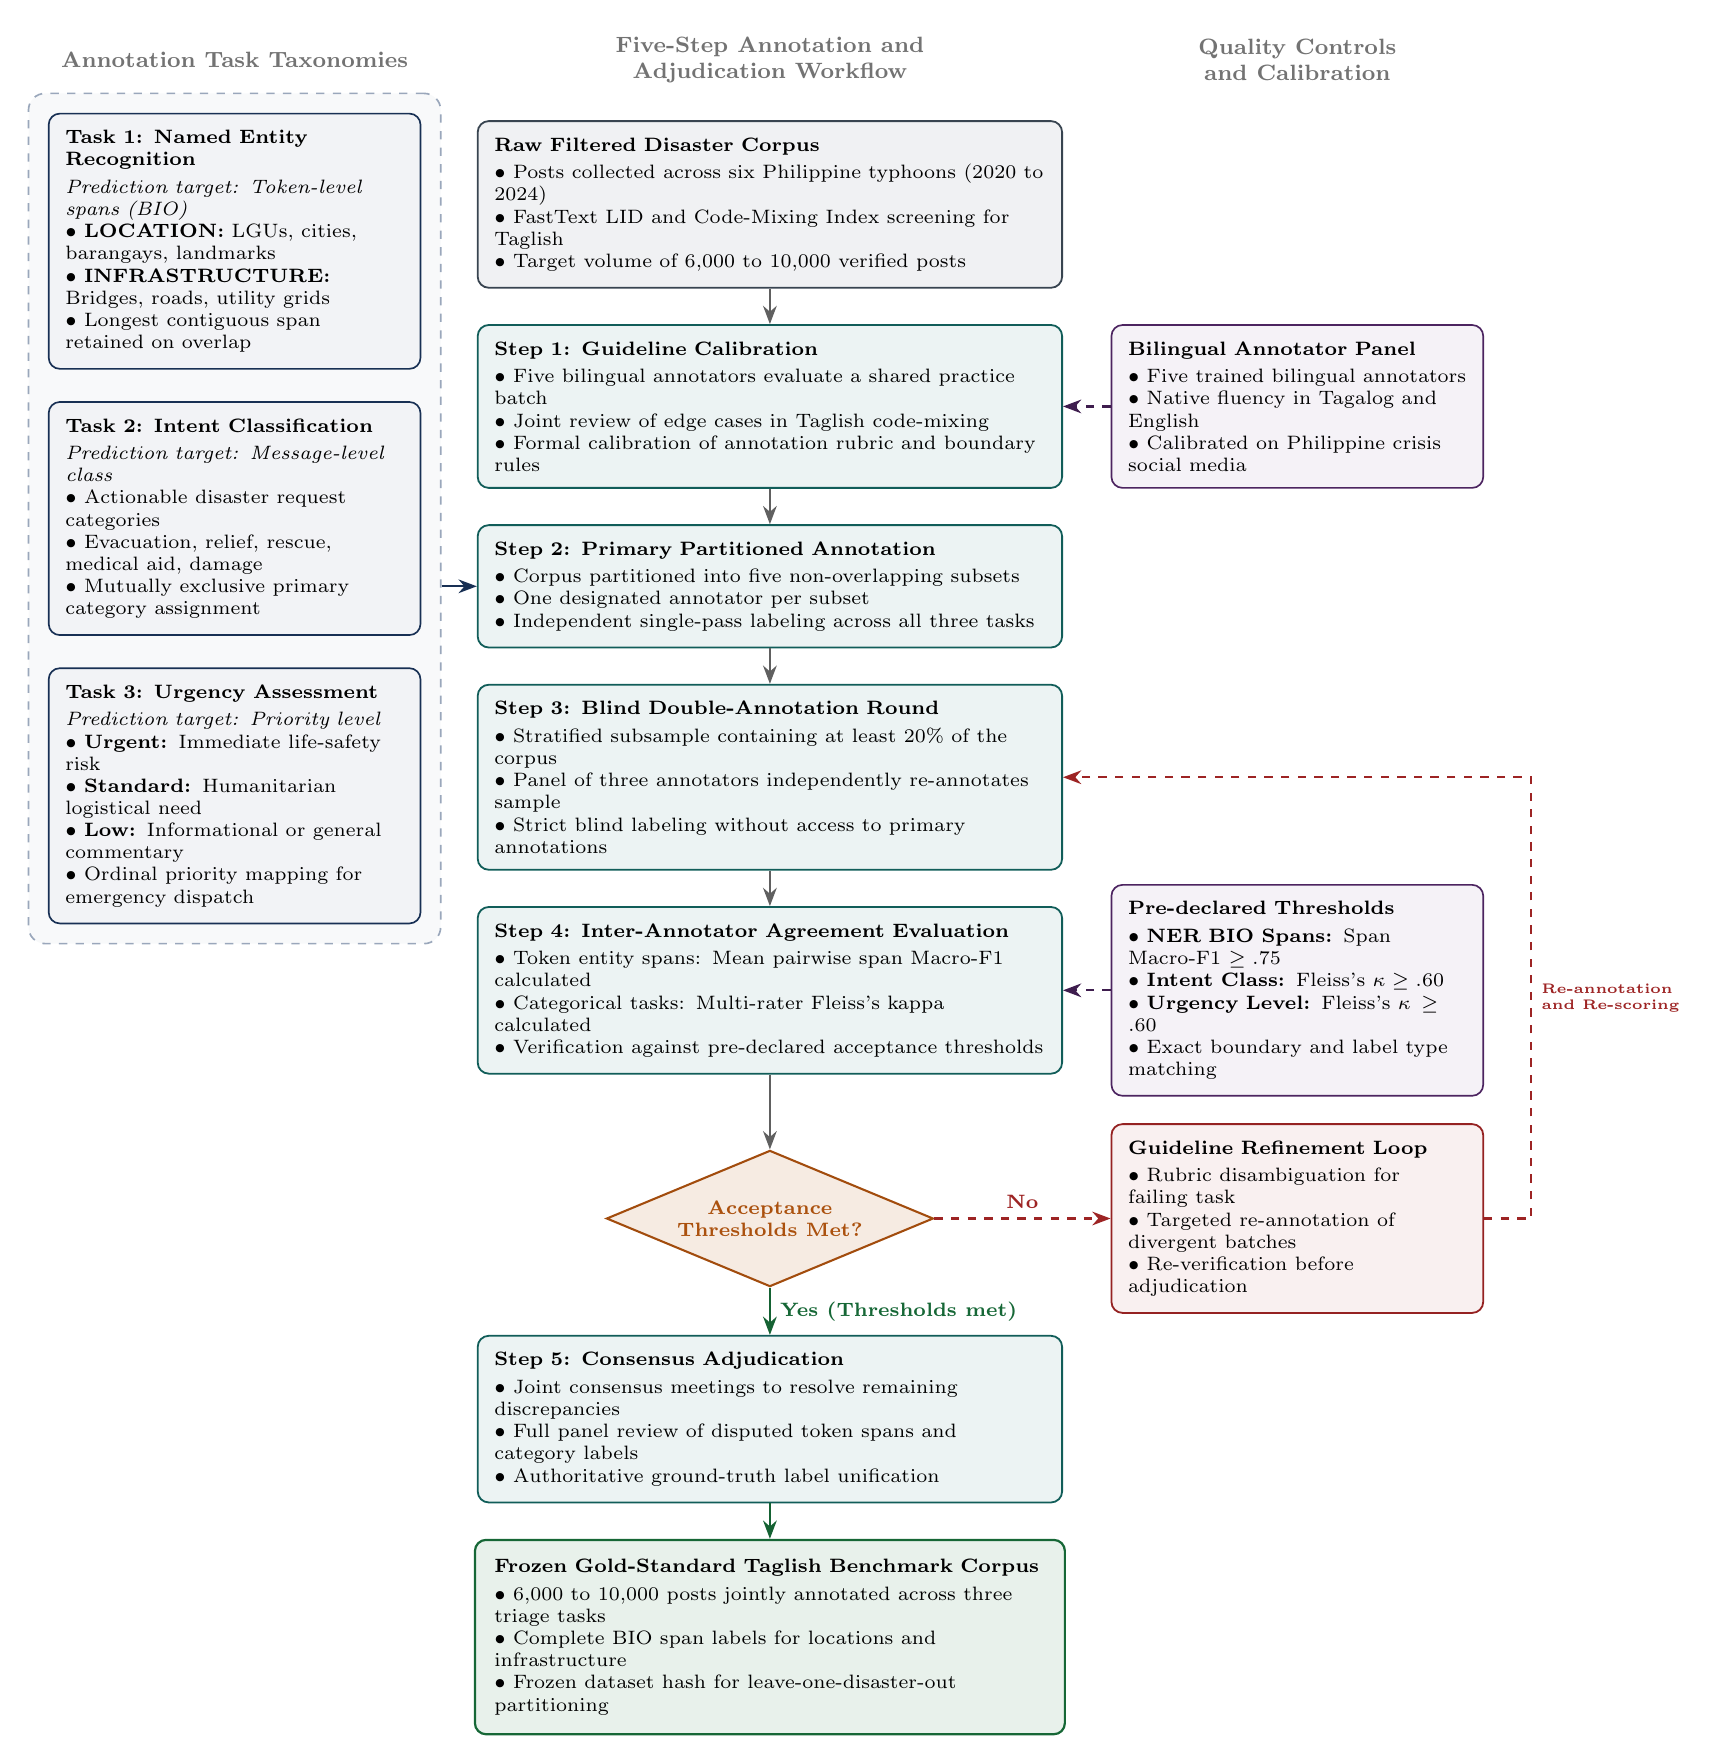
\begin{tikzpicture}[
    font=\small,
    >=Stealth,
    every node/.append style={execute at begin node={\hyphenpenalty=10000\exhyphenpenalty=10000\relax}},
    % Styles
    header/.style={
        font=\bfseries\footnotesize,
        text=gray!90!black,
        align=center
    },
    col1card/.style={
        draw=navyblue!80!black,
        fill=navyblue!6,
        rounded corners=4pt,
        align=left,
        inner sep=6pt,
        font=\scriptsize,
        line width=0.6pt,
        text width=4.3cm
    },
    col3card/.style={
        draw=purplecat!80!black,
        fill=purplecat!6,
        rounded corners=4pt,
        align=left,
        inner sep=6pt,
        font=\scriptsize,
        line width=0.6pt,
        text width=4.3cm
    },
    flowstep/.style={
        draw=tealblue!85!black,
        fill=tealblue!8,
        rounded corners=4pt,
        align=left,
        inner sep=6pt,
        font=\scriptsize,
        line width=0.65pt,
        text width=7.0cm
    },
    decision/.style={
        diamond,
        aspect=2.4,
        draw=ambergold!90!black,
        fill=ambergold!12,
        align=center,
        inner sep=3pt,
        font=\scriptsize\bfseries,
        line width=0.75pt,
        text=ambergold!95!black
    },
    finalcorpus/.style={
        draw=forestgreen!90!black,
        fill=forestgreen!10,
        rounded corners=4pt,
        align=left,
        inner sep=7pt,
        font=\scriptsize,
        line width=0.8pt,
        text width=7.0cm
    },
    fallbackcard/.style={
        draw=crimsonred!85!black,
        fill=crimsonred!7,
        rounded corners=4pt,
        align=left,
        inner sep=6pt,
        font=\scriptsize,
        line width=0.65pt,
        text width=4.3cm
    },
    flowarrow/.style={
        ->,
        thick,
        draw=gray!75!black
    },
    looparrow/.style={
        ->,
        thick,
        dashed,
        draw=crimsonred!90!black
    },
    passarrow/.style={
        ->,
        thick,
        draw=forestgreen!85!black
    }
]

    % =========================================================================
    % COLUMN HEADERS
    % =========================================================================
    \node[header, text width=4.5cm] (h1) 
        {Annotation Task Taxonomies};
    \node[header, text width=7.0cm, right=0.8cm of h1] (h2) 
        {Five-Step Annotation and Adjudication Workflow};
    \node[header, text width=4.3cm, right=0.8cm of h2] (h3) 
        {Quality Controls and Calibration};

    % =========================================================================
    % CENTER COLUMN: WORKFLOW STEPS
    % =========================================================================

    % Input Data Corpus
    \node[flowstep, below=0.35cm of h2, draw=slategrey!80!black, fill=slategrey!8] (s0) {
        \textbf{Raw Filtered Disaster Corpus}\\[2pt]
        $\bullet$ Posts collected across six Philippine typhoons (2020 to 2024)\\
        $\bullet$ FastText LID and Code-Mixing Index screening for Taglish\\
        $\bullet$ Target volume of 6,000 to 10,000 verified posts
    };

    % Step 1: Guideline Calibration
    \node[flowstep, below=0.45cm of s0] (s1) {
        \textbf{Step 1: Guideline Calibration}\\[2pt]
        $\bullet$ Five bilingual annotators evaluate a shared practice batch\\
        $\bullet$ Joint review of edge cases in Taglish code-mixing\\
        $\bullet$ Formal calibration of annotation rubric and boundary rules
    };

    % Step 2: Production Annotation
    \node[flowstep, below=0.45cm of s1] (s2) {
        \textbf{Step 2: Primary Partitioned Annotation}\\[2pt]
        $\bullet$ Corpus partitioned into five non-overlapping subsets\\
        $\bullet$ One designated annotator per subset\\
        $\bullet$ Independent single-pass labeling across all three tasks
    };

    % Step 3: Double Annotation
    \node[flowstep, below=0.45cm of s2] (s3) {
        \textbf{Step 3: Blind Double-Annotation Round}\\[2pt]
        $\bullet$ Stratified subsample containing at least 20\% of the corpus\\
        $\bullet$ Panel of three annotators independently re-annotates sample\\
        $\bullet$ Strict blind labeling without access to primary annotations
    };

    % Step 4: Agreement Verification
    \node[flowstep, below=0.45cm of s3] (s4) {
        \textbf{Step 4: Inter-Annotator Agreement Evaluation}\\[2pt]
        $\bullet$ Token entity spans: Mean pairwise span Macro-F1 calculated\\
        $\bullet$ Categorical tasks: Multi-rater Fleiss's kappa calculated\\
        $\bullet$ Verification against pre-declared acceptance thresholds
    };

    % Decision Diamond (Spaced to align cleanly with q3)
    \node[decision, below=0.95cm of s4] (dec) {
        Acceptance\\
        Thresholds Met?
    };

    % Step 5: Consensus Adjudication
    \node[flowstep, below=0.6cm of dec] (s5) {
        \textbf{Step 5: Consensus Adjudication}\\[2pt]
        $\bullet$ Joint consensus meetings to resolve remaining discrepancies\\
        $\bullet$ Full panel review of disputed token spans and category labels\\
        $\bullet$ Authoritative ground-truth label unification
    };

    % Output Gold Standard Corpus
    \node[finalcorpus, below=0.45cm of s5] (sout) {
        \textbf{Frozen Gold-Standard Taglish Benchmark Corpus}\\[2pt]
        $\bullet$ 6,000 to 10,000 posts jointly annotated across three triage tasks\\
        $\bullet$ Complete BIO span labels for locations and infrastructure\\
        $\bullet$ Frozen dataset hash for leave-one-disaster-out partitioning
    };

    % =========================================================================
    % LEFT COLUMN: TARGET TAXONOMIES
    % =========================================================================

    % Task 1: NER (Chained below h1)
    \node[col1card, below=0.45cm of h1] (t1) {
        \textbf{Task 1: Named Entity Recognition}\\[2pt]
        \textit{Prediction target: Token-level spans (BIO)}\\
        $\bullet$ \textbf{LOCATION:} LGUs, cities, barangays, landmarks\\
        $\bullet$ \textbf{INFRASTRUCTURE:} Bridges, roads, utility grids\\
        $\bullet$ Longest contiguous span retained on overlap
    };

    % Task 2: Intent Classification (Chained below t1)
    \node[col1card, below=0.4cm of t1] (t2) {
        \textbf{Task 2: Intent Classification}\\[2pt]
        \textit{Prediction target: Message-level class}\\
        $\bullet$ Actionable disaster request categories\\
        $\bullet$ Evacuation, relief, rescue, medical aid, damage\\
        $\bullet$ Mutually exclusive primary category assignment
    };

    % Task 3: Urgency Assessment (Chained below t2)
    \node[col1card, below=0.4cm of t2] (t3) {
        \textbf{Task 3: Urgency Assessment}\\[2pt]
        \textit{Prediction target: Priority level}\\
        $\bullet$ \textbf{Urgent:} Immediate life-safety risk\\
        $\bullet$ \textbf{Standard:} Humanitarian logistical need\\
        $\bullet$ \textbf{Low:} Informational or general commentary\\
        $\bullet$ Ordinal priority mapping for emergency dispatch
    };

    % Background container for Left Column Schemas
    \begin{scope}[on background layer]
        \node[draw=navyblue!45, fill=navyblue!3, rounded corners=6pt, dashed, line width=0.6pt, 
              fit=(t1)(t2)(t3), inner sep=7pt] (box_tasks) {};
    \end{scope}

    % =========================================================================
    % RIGHT COLUMN: QUALITY CONTROLS & FEEDBACK
    % =========================================================================

    % Annotator Panel Card (Aligned with Step 1)
    \node[col3card] (q1) at (h3 |- s1) {
        \textbf{Bilingual Annotator Panel}\\[2pt]
        $\bullet$ Five trained bilingual annotators\\
        $\bullet$ Native fluency in Tagalog and English\\
        $\bullet$ Calibrated on Philippine crisis social media
    };

    % Agreement Thresholds Card (Aligned with Step 4)
    \node[col3card] (q2) at (h3 |- s4) {
        \textbf{Pre-declared Thresholds}\\[2pt]
        $\bullet$ \textbf{NER BIO Spans:} Span Macro-F1 $\ge .75$\\
        $\bullet$ \textbf{Intent Class:} Fleiss's $\kappa \ge .60$\\
        $\bullet$ \textbf{Urgency Level:} Fleiss's $\kappa \ge .60$\\
        $\bullet$ Exact boundary and label type matching
    };

    % Fallback Revision Card (Aligned with Decision Diamond)
    \node[fallbackcard] (q3) at (h3 |- dec) {
        \textbf{Guideline Refinement Loop}\\[2pt]
        $\bullet$ Rubric disambiguation for failing task\\
        $\bullet$ Targeted re-annotation of divergent batches\\
        $\bullet$ Re-verification before adjudication
    };

    % =========================================================================
    % CONNECTING ARROWS
    % =========================================================================

    % Main vertical flow
    \draw[flowarrow] (s0) -- (s1);
    \draw[flowarrow] (s1) -- (s2);
    \draw[flowarrow] (s2) -- (s3);
    \draw[flowarrow] (s3) -- (s4);
    \draw[flowarrow] (s4) -- (dec);
    \draw[passarrow] (dec) -- node[right, font=\scriptsize\bfseries, text=forestgreen!90!black] {Yes (Thresholds met)} (s5);
    \draw[passarrow] (s5) -- (sout);

    % SINGLE Clean Horizontal Arrow from Schema Container into Step 2
    \draw[flowarrow, thick, draw=navyblue!80!black] (box_tasks.east |- s2.west) -- (s2.west);

    % Cross-links from right column (Controls into Steps)
    \draw[flowarrow, dashed, draw=purplecat!65!black] (q1.west) -- (s1.east);
    \draw[flowarrow, dashed, draw=purplecat!65!black] (q2.west) -- (s4.east);

    % Negative branch: Decision to Refinement Loop (Horizontal)
    \draw[looparrow] (dec.east) -- node[above, font=\scriptsize\bfseries, text=crimsonred!90!black] {No} (q3.west);

    % Feedback arrow from Refinement Loop routing around the right side back up to Step 3
    \draw[looparrow] (q3.east) -- ++(0.6, 0) |- node[pos=0.25, right, font=\tiny\bfseries, text=crimsonred!90!black, align=left] {
        Re-annotation\\
        and Re-scoring
    } ($(s3.east) + (0.3, 0)$) -- (s3.east);

\end{tikzpicture}
\end{document}
